\chapter{Introduction}
\label{ch1}

%%%%% https://cerncourier.com/a/pushing-the-precision-frontier/
% https://home.cern/news/news/physics/why-precision-luminosity-measurements-matter
Particle physics is the branch of physics that focuses on studying the fundamental particles and forces that make up matter and radiation in the universe. The Standard Model classifies the fundamental particles and their interactions as fermions, which are matter particles, and bosons, which are force-carrying particles. High-energy particle accelerators are used to study these interactions by measuring various parameters and properties of the particles produced during collisions. This chapter provides a brief overview of elementary particles, particle colliders, and the measurement of their performance. It emphasizes the concepts and definitions necessary for understanding this thesis project.

\section{Particle Physics and The Standard Model}

The universe is composed of several different particles. Atoms are bound states of negatively charged electrons $(e^{-})$, which orbit around a central nucleus consisting of positively charged protons $(p)$ and electrically neutral neutrons $(n)$. The electrons are bound to the nucleus by the electrostatic attraction between opposite charges, while the protons and neutrons are held together by the strong nuclear force. Completing the fundamental interactions of particle physics are the weak force and gravity. The weak force is responsible for nuclear $\beta$ decays and nuclear fusion, while gravity, although extremely weak, is always attractive and therefore responsible for the large-scale structure in the universe.
While this is a simple physical model, at higher energy scales, more complex structures are observed, leading to the discovery of 17 fundamental particles that make up our entire universe. These particles are divided into two groups: fermions with spin $1/2$ and bosons with integer spin \cite{thomson_2013}.\\

Fermions are the particles that constitute matter, consisting of twelve fundamental particles classified into two types: leptons and quarks. These particles are further divided into three generations, with each member of a higher generation having a greater mass than the corresponding particle of the previous generation. The six leptons include three charged particles: electron ($e$\textsuperscript{-}), muon (${\mu}$\textsuperscript{-}), and tau (${\tau}$\textsuperscript{-}), as well as their corresponding neutrinos: electron-neutrino ($\nu_{e}$), muon-neutrino ($\nu_{\mu}$), and tau-neutrino ($\nu_{\tau}$). Quarks, on the other hand, can only be found in particles called hadrons. The group of quarks consists of the up quark ($u$), down quark ($d$), charm quark ($c$), strange quark ($s$), top quark ($t$), and bottom quark ($b$) \cite{griff,thomson_2013}. The properties of these twelve particles are summarized in Table \ref{tab:table1}.

\begin{table}[h!]
	\begin{center}
%\centering
	\caption{The twelve fundamental fermions divided into quarks and leptons.\
The masses of the quarks are the current masses \cite{thomson_2013}.}
		\label{tab:table1}
		\begin{tabular}{lllrcllrc}
                                                                                & \multicolumn{4}{c}{\textbf{Leptons}}                                                                     & \multicolumn{4}{c}{\textbf{Quarks}}                                                \\ 
%\cline{2-9}
 \midrule[1.1pt]
                            \multicolumn{1}{c}{Generation }& \multicolumn{2}{c}{Particle } & \multicolumn{1}{c}{\textit{Q}} & mass/GeV                          & \multicolumn{2}{c}{Particle} & \multicolumn{1}{c}{\textit{Q}} & mass/GeV  \\ 
\hline
\multirow{2}{*}{\begin{tabular}[c]{@{}l@{}}First\end{tabular}}  & electron & ($e$\textsuperscript{-})                 & -1                             & 0.0005                            & down    & ($d$)                & -1/3                           & 0.003     \\
                                                                                & $e$-neutrino & ($\nu_{e}$)                 & 0                              & \textless{}10\textsuperscript{-9} & up      & ($u$)                & +2/3                           & 0.005     \\
\multirow{2}{*}{\begin{tabular}[c]{@{}l@{}}Second\end{tabular}} & muon     & (${\mu}$\textsuperscript{-})                 & -1                             & 0.106                             & strange & ($s$)                & -1/3                           & 0.1       \\
                                                                                & $\mu$-neutrino & ($\nu_{\mu}$)                 & 0                              & \textless{}10\textsuperscript{-9} & charm   & ($c$)                & +2/3                           & 1.3       \\
\multirow{2}{*}{\begin{tabular}[c]{@{}l@{}}Third\end{tabular}} & tau      & ({$\tau}$\textsuperscript{-})                 & -1                             & 1.78                              & bottom  & ($b$)                & -1/3                           & 4.5       \\
                                                                                & $\tau$-neutrino & ($\nu_{\tau}$)                 & 0                              & \textless{}10\textsuperscript{-9} & top     &($t$)                & +2/3                           & 174      
\end{tabular}
	\end{center}
		\end{table}

The bosons are responsible for describing the interactions between fermions through the exchange of particles. These exchange particles are known as gauge bosons and include the photon $\gamma$ for electromagnetic force, $W^{\pm}$ and $Z^{0}$ for the weak force and gluons $g$ for the strong force \cite{thomson_2013}. Additionally, there is a scalar boson called the "Higgs boson", which is associated with the mechanism that gives mass to all fundamental particles. The forces experienced by fermions can be seen in table  \ref{tab:table2}.

\begin{table}[h!]
  \begin{center}
    \caption{Force experienced by the fermions \cite{thomson_2013}.}
    \label{tab:table2}
    \begin{tabular}{l c c c c}
    &    &  \textbf{Electromagnetic} & \textbf{Weak} & \textbf{Strong}\\
      \midrule[1.1pt]
      \multirow{2}{*}{Leptons} & ${e}$\textsuperscript{-} \hspace{0.3cm}  ${\mu}$\textsuperscript{-} \hspace{0.3cm} ${\tau}$\textsuperscript{-} & \checkmark & \checkmark & \\ % <-- Combining 2 rows with arbitrary with (*) and content 12
      & $ \nu_{e} $ \hspace{0.3cm}  $\nu_{\mu}$ \hspace{0.3cm} $\nu_{\tau}$  &  & \checkmark\\ % <-- Content of first column omitted.
      \hline
      \multirow{2}{*}{Quarks} & $u$ \hspace{0.5cm}  $c$\hspace{0.5cm} $t$ & \checkmark & \checkmark& \checkmark\\
      & $d$ \hspace{0.5cm}  $s$\hspace{0.5cm} $b$ & \checkmark & \checkmark & \checkmark\\

    \end{tabular}
  \end{center}
\end{table}

All of these particles are described by the Standard Model (SM), which is the best theoretical model to date for providing a successful description of experimental data. However, most of this data comes from particle colliders since these particles can only be produced and studied through collisions at high energy.

\section{Particle Colliders and production cross section}

Most of the recent breakthroughs in particle physics have resulted from experiments conducted at high-energy particle accelerators. These accelerators are the most powerful microscopes for observing the tiniest inner structures of cells, genes, molecules, atoms, and their constituent particles such as protons, neutrons, electrons, neutrinos, and quarks. Moreover, they may also help discover yet unknown fundamental building blocks of the universe, such as dark matter and dark energy.\\

Particle colliders produce and accelerate beams of charged particles at high speeds (close to the speed of light) using electromagnetic fields; the high-energy collisions of these beams produce individual interactions referred to as events. These collisions produce massive particles, such as the Higgs boson or the top quark. These particles  cannot be observed directly, almost immediately they transform (or decay) into lighter particles, which in turn also decay. They are measured and identified by a wide range of experiments (particle detectors), whose technologies, techniques and designs are based on the properties of the particles and on the nature of their interactions with matter \cite{thomson_2013}.\\

In general, particle detector is typically constructed as a cylindrical or polygonal barrel section, oriented parallel to the incoming colliding beams. Two flat end caps seal the cylindrical structure, ensuring nearly complete solid angle coverage all the way down to the beam pipe. This detector comprises multiple layers, each designed to detect the different particles generated during collisions \cite{thomson_2013}.\\

The performance of particle colliders is typically evaluated based on two parameters: the beam energy and the luminosity. The available energy for producing new effects is one of the most important parameters, as it determines the types of particles that can be studied or discovered. In these experiments, particles are accelerated and two beams are brought together at an intersection point where they collide.\\

Colliding beam machines have the advantage that they can achieve much higher centre-of-mass energies, at various points the beams intersect and scattering takes place. If the incident particles have the same energy (equal mass) and therefore equal but opposite momentum, then the experiment is taking place in the centre-of-mass (CM) frame and the full energy delivered by the accelerator, can be used to produce high mass particles  \cite{undergraduate_accelerators_chapter}.
In particle physics the Lorentz invariant quantity $s$ denote the square of the total incoming energy and is defined as: 
\begin{equation}
s = \left ( \sum_{i = 1,2}^{}E_{i} \right )^{2}-\left ( \sum_{i = 1,2}^{}p_{i} \right )^{2}c^{2}
\end{equation}
Where $E$ and \textbf{$p$}  are the energy and the momenta of each incoming particle respectively, in the CM frame, where the momenta are equal and opposite, the second term vanishes and  $s = 4E^2$.\\

The second important parameter of the collider's performance is the luminosity, defined as the  quantity that measures the ability of a particle accelerator to produce the required number of interactions and is the proportionality factor  between the number of events of particular physics process per second $dR/dt$ and the quantum mechanical probability for the interaction called cross section \sigma_{p} \cite{ref_lib_vol3}.\\

The technical meaning of "cross section" in particle physics is quite different from its common usage, while "cross section" typically refers to a slice of an object, in particle physics, it often refers to the probability that two particles will collide and react in a specific manner. When two beams cross in a particle accelerator, a variety of different processes can occur and  the cross section of a given process depends on the type and energy of the colliding particles.
At the Large Hadron Collider (LHC), certain particles such as  $W^{\pm}$ and $Z^{0}$ bosons have large cross sections , making their observation more frequent, while the production of a Higgs boson has a much lower cross section, making it more difficult to produce \cite{thomson_2013}.\\

To show better this concept, we present the most simplest scenario, where a beam of particles of type $a$, with a flux denoted by $\phi_{a}$, passes through a region of space containing $n_{b}$ particles per unit volume of type $b$. The interaction rate per target particle $r_{b}$ is proportional to the incident particle flux and can be expressed as follows \cite{thomson_2013}:

\begin{equation*}
  r_{b}=\sigma \phi_{a}
\end{equation*}

The essence of fundamental physics is encapsulated in $\sigma$, which has units of area and is referred to as the interaction cross section. It can be useful to conceptualize $\sigma$ as the effective cross-sectional area associated with each target particle, in general, the cross section merely represents the underlying quantum mechanical likelihood that an interaction will occur \cite{thomson_2013}. The definition of the cross section is illustrated in Figure \ref{cross_section}(a), where a single incident particle of type $a$ is travelling with a velocity $v_{a}$ in a region defined by the area $A$, wish contains $n_{b}$ particles of type $b$ per unit volume moving with a velocity $v_{b}$ in the opposite direction to $v_{a}$. 

\begin{center}
  \begin{figure}[h!]
    \centering
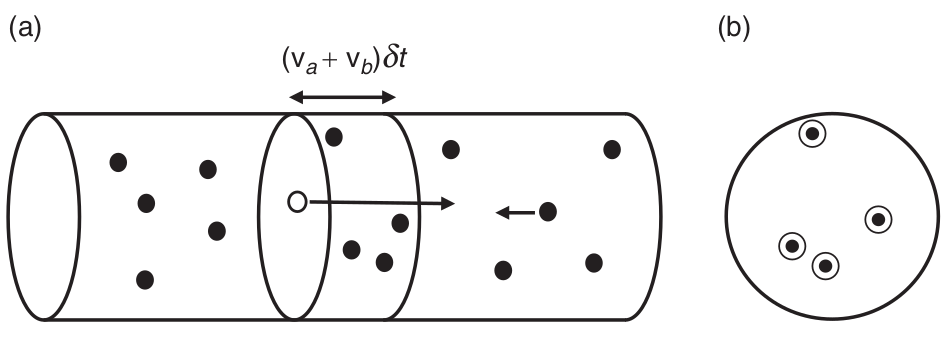
\includegraphics[scale=.35]{Chapter1/cross_section.png} 
 \caption[Cross section illustration]{Left hand (a): single incident particle of type $a$ traversing a region containing particles of type $b$. Right-hand plot (b): projected view of the region traversed by the incident particle in time $\delta t$ \cite{thomson_2013}.}
    \label{cross_section}
  \end{figure}
\end{center}

In  a time $\delta t$, the particle $a$  crosses a region containing $\delta N= nb(v_{a}+v_{b}) A \delta t$ of type $b$. The interaction probability can be obtained from the $effective$ total cross sectional area of the $\delta N$ particles divided by the area $A$, which can be thougth of as the probability that the incident particle passes through one of the regions of area $\sigma$ drawn around each of the $\delta N$ target particles, as shown in Fig. \ref{cross_section}(b). For a beam of particles of type $a$ with number density $n_{a}$ confined to a volume $V$, the total interaction rate is $\text{rate}=(n_{a}v)(n_{b}V) \sigma = \phi N_{b} \sigma$,  more formally, the cross section for a process is defined as \cite{thomson_2013}:

\begin{equation}
\sigma=\frac{\text{number of interaction per unit time per target particle}}{\text{incident flux}}
\end{equation}

Where the flux $\phi$ accounts for the relative motion of particles.
The value of the cross section is crucial as it represents the constant of proportionality between the rate measured by the detector and the luminosity.

%begin{equation}
%\sigma=\frac{\text{number of interaction per unit time per target particle}}{\text{incident flux}}
%\end{equation}

%\delta P= \frac{\delta N \sigma}{A}=\frac{n_{b}(v_{a}+v_{b})A\sigma \dela t}{A}= n_{b}v\sigma \delta t$
%where $v=v_{a}+v_{b}$. The interaction rate for each particle of type $a$ is $r_{a}= \frac{dP}{dt}= n_{b} v\sigma$.
%For a beam of particles of type $a$ with number density $n_{a}$ confined to a volume $V$, the total interaction rate is:
%$\text{rate}=r_{a}n_{a}V=(n_{b}v\sigma) n_{a}V= (n_{a}v)(n_{b}V)\sigma$

%$\text{rate}=(n_{a}v)(n_{b}V) \sigma = \phi N_{b} \sigma$

%Thus the total rate is equal to
%$\text{rate}= \text{flux} \times \text{number of target particles} \times \text{cross section}$

%More formally, the cross section for a process is defined as:
\section{Luminosity }

In particle physics experiments besides the energy, the number of useful interactions (events) is the most important parameter. The quantity that measures the ability of a particle accelerator to produce these interactions is called instantaneous luminosity $\mathcal{L}_{inst}$ and is the proportionality factor between the number of events per second ($dR/dt$) and the cross section $\sigma_{p}$ \cite{concept_of_luminosity}: 

\begin{equation}
\frac{dR}{dt}=\mathcal{L}_{inst} \cdot \sigma_{p}
\end{equation}

Where the unit of luminosity is $cm^{-2}s^{-1}$. 

To derive a general expression for luminosity in the case of two colliding beams, we consider both beams to serve as the target and the incoming beam simultaneously. We will assume that the beams are "bunched", meaning that the particles are grouped into packets or bunches. 

\begin{center}
  \begin{figure}[h!]
    \centering
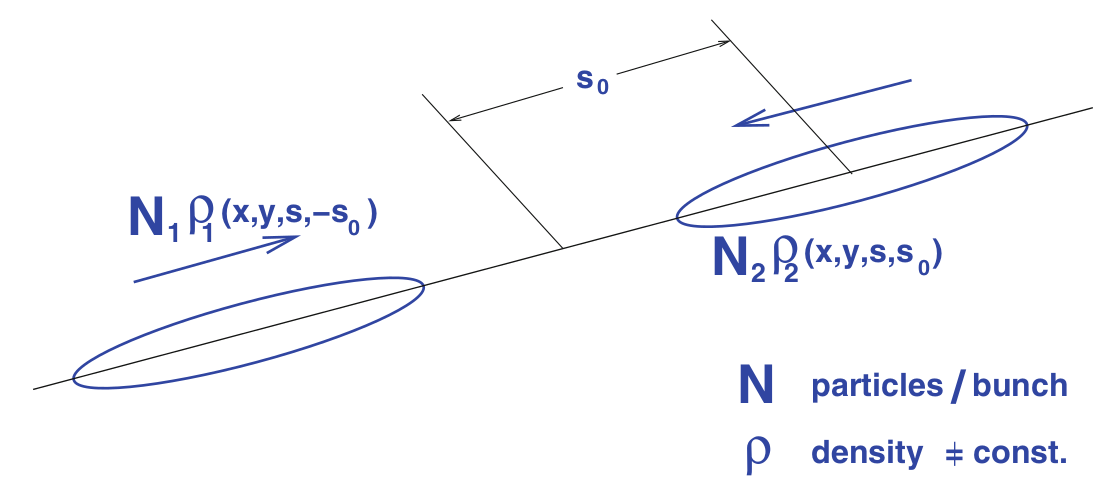
\includegraphics[scale=.25]{Chapter1/luminosity.png} 
 \caption[Colliding beam interaction]{Schematic view of a colliding beam interaction\cite{concept_of_luminosity}}
    \label{luminosity}
  \end{figure}
\end{center}

A schematic picture is shown in Fig. \ref{luminosity}. Since the two beams are not stationary but are moving through each other, the overlap integral depends on the longitudinal position of the bunches, and therefore on time. As the beams move towards and through each other, the two beams have different distribution functions and a different number of particles in the beams \cite{concept_of_luminosity}. The overlap integral, which is proportional to the luminosity $\mathcal{L}_{inst}$, can then be written as:
 
\begin{equation}
  \mathcal{L}_{inst}\propto K\cdot \int\int \int_{-\infty}^{\infty} \rho_{1}(x,y,s,-s_{0}) \rho_{2}(x,y,s,s_{0})dxdydsds_{0}
    \label{lumi_1}
\end{equation}
 
Where  $\rho_{1}(x,y,s,-s_{0})$ and $\rho_{2}(x,y,s,s_{0})$ are the time dependent beam density distribution functions. We assume, that the two bunches meet at $s_{0} = 0$. Because the beams are moving against each other, we have to multiply this expression with a relativistic kinematic factor:

\begin{equation}
 K = \sqrt{(\vec{v_{1}}-\vec{v_{2}})^{2}-(\vec{v_{1}}\times \vec{v_{2}})^{2}/c^{2}}
    \label{kinematic}
\end{equation}

Specifically, in the case of exactly head-on collisions of bunches travelling almost at the speed of light, this factor becomes 2.\\
Assuming uncorrelated densities in all planes and head-on collisions where the velocities of the two bunches are opposite $(\vec{v_{1}}=-\vec{v_{2}})$, the overlap integral can be factorized as:

\begin{equation}
  \mathcal{L}_{inst}= 2N_{b} N_{1}N_{2}f \int\int\int\int_{-\infty}^{\infty}  \rho_{1x}(x)\rho_{1y}(y)\rho_{1s}(s-s_{0})\rho_{2x}(x)\rho_{2y}(y)\rho_{2s}(s+s_{0}) dxdydsds_{0}
    \label{luminosity_2}
\end{equation}

where $N_{1}$ and $N_{2}$ are the particles per bunch, $f$ the revolution frequency and $N_{b}$ is the number of bunches in one beam.\\



%\begin{eqnarray}
%\rho_{iz}(z)= \frac{1}{\sqrt{2\pi} \sigma_{z}} exp \biggl(-\frac{z^{2}}{2\sigma_{z}^{2}} \biggr)&z=x,y&i=1,2 
%\end{eqnarray}

%\begin{eqnarray}
%\rho_{s}(s\pm s_{0})= \frac{1}{\sqrt{2\pi} \sigma_{s}} exp \biggl(-\frac{(s\pm s_{0})^{2}}{2\sigma_{s}^{2}} \biggr)
%\end{eqnarray}

Assuming Gaussian profiles in all dimensions and approximately equal bunch lengths $(\sigma_{1s}\approx \sigma_{2s})$, the equation \ref{luminosity_2} can be solved.
For a general case where $\sigma_{1x}\neq \sigma_{2x} \text{ and } \sigma_{1y}\neq \sigma_{2y}$

\begin{equation}
  \mathcal{L}_{inst}= \frac{N_{1} N_{2} N_{b}f }{2\pi \sqrt{\sigma_{1x}^{2}+\sigma_{2x}^{2}}\sqrt{\sigma_{2y}^{2}+\sigma_{2y}^{2}}}
  \label{lumi_general}
\end{equation}

For a specific case, asuming equal beams, $\sigma_{1x}= \sigma_{2x} ,\sigma_{1y}= \sigma_{2y}$:

\begin{equation}
  \mathcal{L}_{inst}= \frac{N_{1} N_{2} N_{b}f }{4\pi \sigma_{x} \sigma_{y}}
  \label{lumi_theor}
\end{equation}

This is the well known expression for the luminosity of two Gaussian beams colliding head-on. It shows how the luminosity depends on the number of particles per bunch and the beam sizes \cite{concept_of_luminosity}.

In practice,the integral in  \ref{luminosity_2} cannot be solved analytically because   the properties of the colliding beams are not know precisely, so a experimental technique is implemented with a dedicated machine setup to estimate the integrals, yielding a similar expression as \ref{lumi_theor}.

In order to evaluate the total number of events we use integrated luminosity,it is a measurement of the collected data size, and it is an important value to characterize the performance of an accelerator, defined as \cite{concept_of_luminosity}:

\begin{equation}
  \mathcal{L}_{int}=\int_{0}^{T} \mathcal {L}_{\text{inst}}(t') dt'
\end{equation}

Where the value of $\mathcal{L}_{inst}$ is evaluated over time $T$ (excluding possible dead time) because its intensity decreases as the number of protons reduces during the collisions of the fill. So $\mathcal{L}_{int}$ is directly related to the number of observed events as:

\begin{equation}
  \mathcal{L}_{int} \ndot \sigma_{p}= \text{number of events of interest}
\end{equation}

The integrated luminosity has units of $cm^{-2}$ and is often expressed in inverse barn ($1 barn= 10^{-24}cm^{2}$). \\

Understanding luminosity with the best possible precision is crucial for physics analyses such as searches for new particles, rare processes, or measurements of known particle properties \cite{lumi_motiv}.
The experimental techniques to determine signal rates are mature enough, where the understanding of acceptances, detector biases, reconstruction efficiencies, or background subtraction is at the sub-percent level, so that the final precision of the physics measurement is dominated by the luminosity uncertainty \cite{lumi_paper_def_and_concept}. Ultimately, the greater the precision of the luminosity measurement, the more physicists can understand their observations and delve into hidden corners beyond our current knowledge.

\section{The Large Hadron Collider}

The Large Hadron Collider (LHC) is the world’s largest and most powerful particle accelerator. It first started up on 10 September 2008, and remains the latest addition to CERN’s accelerator complex. The LHC consists of a 27-kilometre ring of superconducting magnets with a number of accelerating structures to boost the energy of the particles along the way. Inside the accelerator, two high-energy particle beams travel at close to the speed of light before they are made to collide. The beams travel in opposite directions in separate beam pipe where the two tubes kept at ultrahigh vacuum. They are guided around the accelerator ring by a strong magnetic field maintained by superconducting electromagnets, these are built from coils of special electric cable that operates in a superconducting state, efficiently conducting electricity without resistance or loss of energy. This requires chilling the magnets to 271.3°C  a temperature colder than outer space \cite{LHC}.\\ 

Magnets of different varieties and sizes are used to direct the beams around the accelerator. These include 1232 dipole magnets, 15 metres in length, which bend the beams, and 392 quadrupole magnets, each 5–7 metres long, which focus the beams. Just prior to collision, another type of magnet is used to "squeeze" the particles closer together to increase the chances of collisions . \\

The production of proton beams for the LHC involves a complex series of pre-acceleration stages. To begin with, hydrogen is ionized to produce protons, which are then accelerated in bunches up to 50 MeV within the Linear Accelerator 2 (LINAC2). Subsequently, these proton bunches are routed through three circular accelerators - the Booster, the Proton Synchrotron (PS), and the Super Proton Synchrotron (SPS)  in order to gradually increase their energy levels to 1.4 GeV, 26 GeV, and 450 GeV, respectively. Following these pre-acceleration stages, the proton bunches are injected into the LHC ring where they are accelerated to reach energies of up to 7 TeV per bunch while circulating in opposite directions. This entire sequence of steps defines a single LHC fill, which typically involves $10^{14}$ protons that are grouped into bunches to form the proton beam. Figure \ref{lhc_com} depicts the complete CERN accelerator complex.

\begin{center}
  \begin{figure}[h]
    \centering
    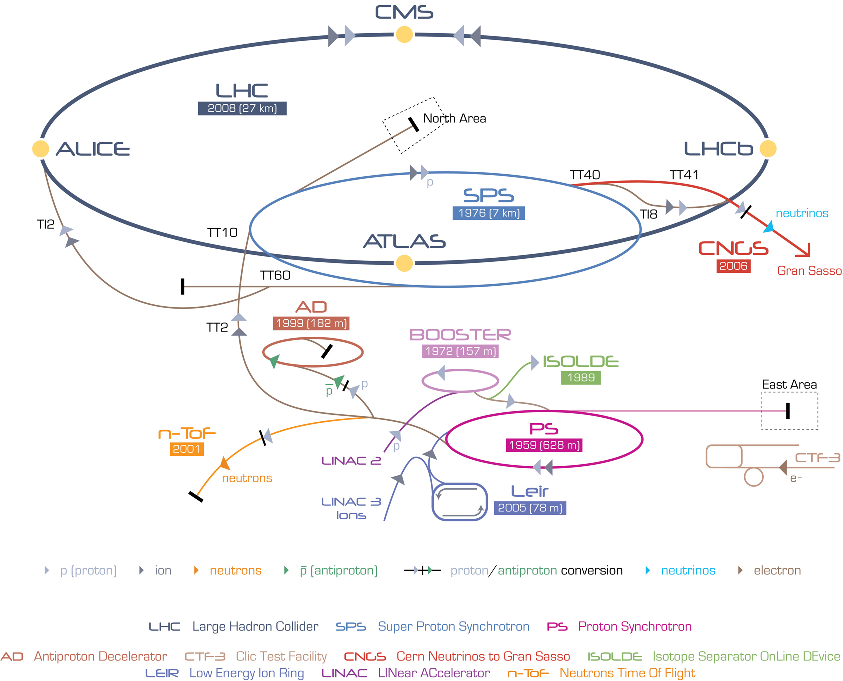
\includegraphics[scale=.45]{Chapter1/lhc_complex_fig.png}
    \caption[LHC Complex]{Diagram of the LCH complex \cite{lhc_complex}.}
    \label{lhc_com}
  \end{figure}
\end{center}

The responsibility for overseeing all controls, services, and technical infrastructure of the LHC lies with the CERN Control Centre. This is the central location where proton beams are directed to collide at four distinct positions along the accelerator ring, corresponding to the positions of the four particle detectors: CMS and ATLAS, which are general-purpose detectors specifically designed to investigate a broad range of Standard Model (SM) and Beyond SM (BSM) physics, while ALICE and LHCb serve as specialized detectors, specifically focused on studying particular phenomena.


\section{Expected  Luminosity precision for LHC Run 3}

Since its inception in 2010 the LHC has undergone three runs and two lengthy shutdowns for maintenance and upgrades. 
Run1 began in 2010 with proton-proton collisions at a center-of-mass energy of $\sqrt{s}=\text{7 TeV}$ and concluded in August 2012 at  $\sqrt{s}=\text{8 TeV}$\cite{LHC_status_2013}. Run 2, which took place at $\sqrt{s}=\text{13 TeV}$, was divided into two stages; the first  occurred from 2015 to 2016, and the second part  was carried out   from 2017 to 2018 \cite{pas_17,pas_18}, efforts are currently underway to further improve the precision of this run. Finally  Run3, which began in 2022 at $\sqrt{s}=\text{13.6 TeV}$ and is currently ongoing. This thesis project aims to contribute to the improvement of the precision of the luminosity for Run 3, where it is expected to obtain an approximate luminosity of $390 fb^{-1}$. \\

The integrated luminosity for each of these runs and years, and their corresponding uncertainty values are presented in table \ref{lumi_values} (luminosity values includes the time from the start of stable beams until the beam is dumped by the LHC), also a visualization of these values measured with CMS is shown in Figure \ref{lumi_per_year_int}, which depicts the delivered luminosity versus time for each year.


\begin{table}[h!]
    \begin{center}
    \caption{Integrated luminosity values recorder by each Run}
	\label{lumi_values}
\begin{tabular}{cccc}
\textbf{Run} & \textbf{Energy $\sqrt{s}$} & \begin{tabular}[c]{@{}c@{}}\textbf{Integrated}\\\textbf{Luminosity}\end{tabular} & \textbf{Precision}    \\ 
\toprule
1(2010-2012) & 8 TeV           & $30 fb^{-1}$                                                                               & 2.5\%                 \\
2(2015-2016) & 13 TeV          & $45.9 fb^{-1}$                                                                             & 1.3\%                 \\
2(2017-2018) & 13 TeV          & $118 fb^{-1}$                                                                              & 2.5\%                 \\
3(2022-2024) & 13.6 TeV        & \begin{tabular}[c]{@{}c@{}}$45 fb^{-1}$(current)\\$390 fb^{-1}$(expected)\end{tabular}                  & \begin{tabular}[c]{@{}c@{}}currently\\estimating  \end{tabular}\\
\end{tabular}
    \end{center}
\end{table}
%%%%%%%%%%%%%%%%%%%%%%%%%%%%%%%%%%%%%%%%%%%
\begin{comment}
\begin{table}[h!]
\begin{center}
    \caption{Integrated luminosity values recorder by each Run}
	\label{lumi_values2}
\begin{tabular}{ccccc}
\multicolumn{1}{l}{\textbf{Run}} & \textbf{Year} & \textbf{Energy $\sqrt{s}$} & \begin{tabular}[c]{@{}c@{}}\textbf{Integrated}\\\textbf{Luminosity}\end{tabular} & \textbf{Precision}    \\ 
\toprule
\multirow{3}{*}{1}               & 2010          & 7 TeV           & $45 pb^{-1}$                                                                                 & 2.5\%                 \\
                                 & 2011          & 7 TeV           & $6.1 fb^{-1}$                                                                                & 2.4\%                 \\
                                 & 2012          & 8 TeV           & $23.3 fb^{-1}$                                                                               & 2.5\%                 \\ 
\hline
\multirow{2}{*}{2}               & 2015          & 13 TeV          & $4.3 fb^{-1}$                                                                              & 1.6\%                 \\
                                 & 2016          & 13 TeV          & $2.6 fb^{-1}$                                                                              & 1.2\%                 \\ 
\hline
\multirow{2}{*}{2}               & 2017          & 13 TeV          & $49.8 fb^{-1}$                                                                             & 2.3\%                 \\
                                 & 2018          & 13 TeV          & $67.9 fb^{-1}$                                                                              & 2.5\%                 \\ 
\hline
\multirow{2}{*}{3}               & 2022          & 13.6 TeV        & $45 fb^{-1}$                                                                                & currently estimating  \\
                                 & 2023          & 13.6 TeV        & currently recording                                                              & currently estimating 
\end{tabular}
 \end{center}
\end{table}
\end{comment}
%%%%%%%%%%%%%%%%%%%%%%%%%%%%%%%%%%%%%%%%%%%%%%
\newpage
  \begin{center}
  \begin{figure}[ht]
    \centering
    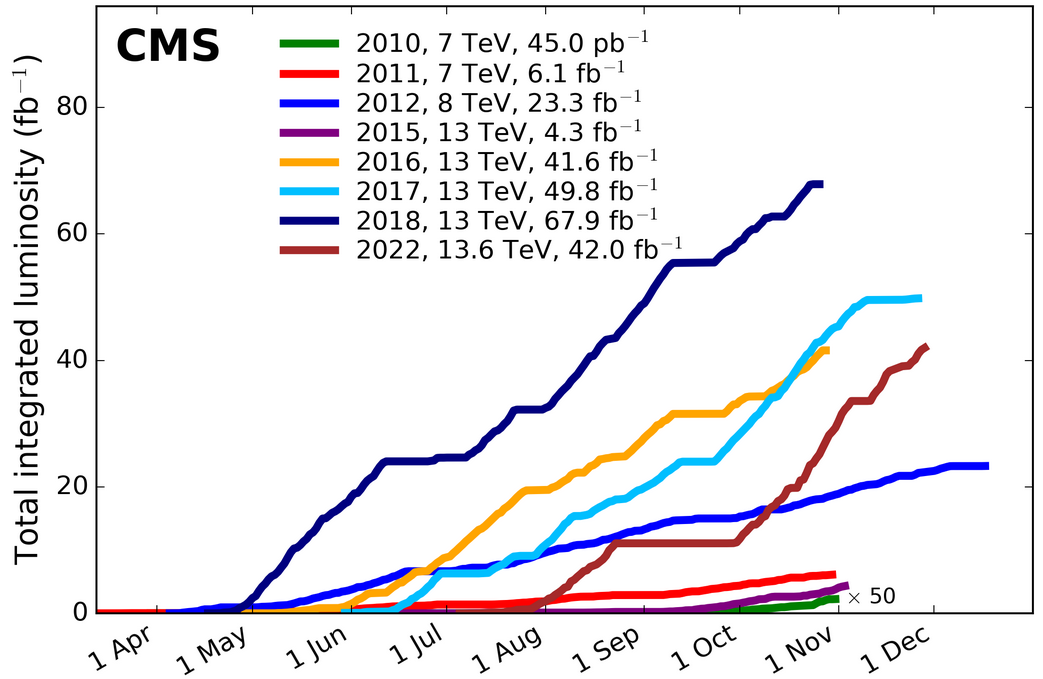
\includegraphics[scale=.28]{Chapter1/int_lumi_per_year.png}
    \caption[CMS Luminosity per year]{Delivered luminosity versus time for Run-1 (2010-2012)\cite{pas_17} and Run-2 (2015-2018)\cite{pas_18} and Run-3 that is still ongoing . Cumulative luminosity versus day delivered to CMS during stable beams for pp collisions at nominal center-of-mass energy.  \cite{wikicern}.}
    \label{lumi_per_year_int}
  \end{figure}
    \end{center}
%% tabla con ano , luminosidad y presicion